\documentclass[12pt]{article}

\usepackage[dvips,letterpaper,margin=0.75in,bottom=0.5in]{geometry}
\usepackage{cite}
\usepackage{slashed}
\usepackage{graphicx}
\usepackage{amsmath}
\usepackage{amssymb}
\usepackage{braket}
\usepackage{pythonhighlight}
\usepackage{mathtools}
\usepackage{tikz}
\begin{document}


\title{PHY 112L \\ Compressing a 2-D Ideal Gas }
\author{Michael Mulhearn}

\maketitle

\section{Ideal Gas in Two Dimensions}

\noindent
For this assignment, we will build a molecular dynamics model for an
ideal gas in two dimensions.  The ideal gas law is:
\begin{equation}
P \, V  = N \, k \, T
\end{equation}
where $P$ is the pressure, $V$ is the volume occupied by the gas, $N$
is the number of molecules in the gas, $k$ is Boltzmann's constant,
and $T$ is the temperature.  The Equipartition theorem, applied to the ideal gas, leads to a total energy of the gas
\begin{equation}
U = \frac{f}{2}NkT
\end{equation}
where $f$ is the number of quadratic degrees of freedom: 3 for an
ideal-gas in 3-D, and 2 for an ideal-gas in 2-D.  The molecules in an
ideal gas have only kinetic energy, and so:
$$U = N\braket{K}$$
where $\braket{K}$ is the average kinetic energy across all molecules, and so:
\begin{equation}
\braket{K} = \frac{f}{2}kT
\end{equation}

In two dimenstions (2-D), the ideal gas law becomes:
\begin{equation}
O \, A  = N \, k \, T
\end{equation}
where $A$ is the area occupied by the gas, and $O$ is the 2-D analog
to pressure: a force per unit length.  We will still call $O$ the
pressure of the 2-D gas.  If one knows the pressure $O$ as a function of the area $A$, then one can calculate the work done on the gas compressing (or expanding) from area $A_1$ to $A_2$ as:
\begin{equation}
W = -\int_{A_1}^{A_2} O(A) \; dA
\end{equation}
The temperature is related to average kinetic energy across all molecules as (setting $f=2$ in the above):
\begin{equation}
\braket{K} = kT.
\end{equation}

\begin{figure}[thb]
\begin{center}
{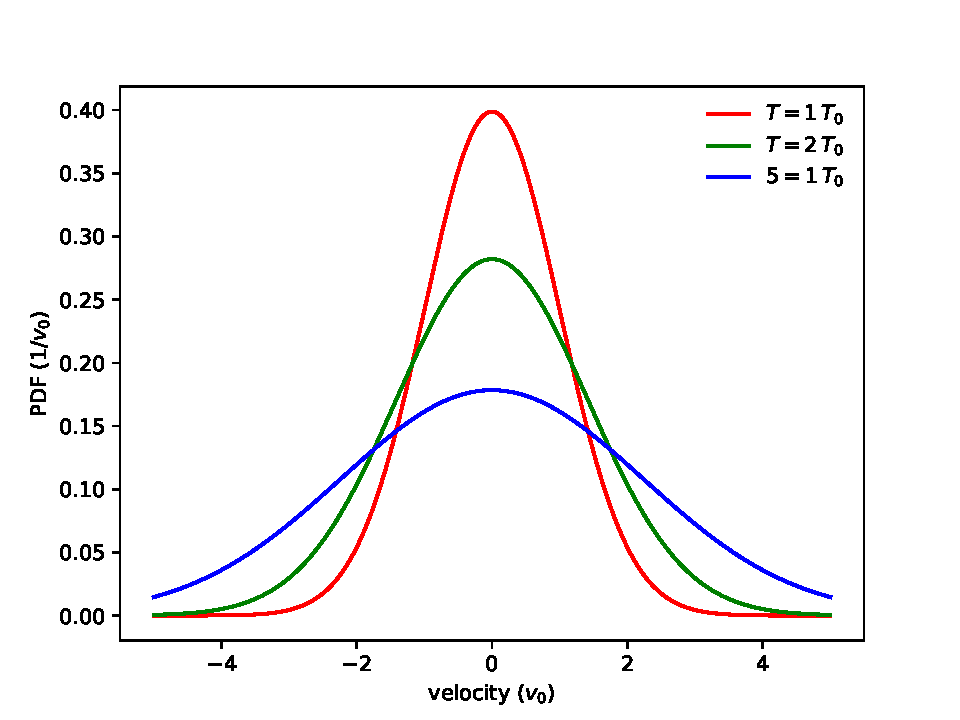
\includegraphics[width=0.60\textwidth]{plots/mbvelocity.pdf}}
\end{center}
\caption{\label{fig:mbvelocity} The PDF for each components of velocity of an ideal gas is a Gaussian distribution.  The corresponding PDF for the speed is the Maxwell-Boltzmann distribution.}
\end{figure}
The probability of finding a particular molecule with kinetic energy:
$$K = \frac{1}{2} mv^2$$
is proptional to the Boltzmann factor for the total energy $E$ of the single molecule:
$$f(v) \; dv \; \propto \; \exp \left(-\frac{E}{kT}\right) dv \; = \; 
\exp \left(-\frac{mv^2}{2kT}\right) dv$$
because for an ideal gas $E=K$.  Properly normalized this is the Maxwell-Boltzmann distribution.
Assuming that the velocity components $v_x$ and $v_y$ are independent random variables, we conclude that:
\begin{equation}
f(v_x) \; dv_x = \left( \frac{m}{2\pi kT} \right)^{1/2} \; \exp \left(-\frac{m v_x^2}{2kT}\right) \; dv_x. 
\end{equation}
with a similar equation for $dv_y$.  This PDF is illustrated in Fig.~\ref{fig:mbvelocity}.

\section{System of Units}

When doing numerical work, it is important to use a well designed
system of units.  Computer programs have limited numerical precision,
so we should never see numbers like
$$k=1.38\times10^{-23} J/K$$ appear in our programs.  Instead, the
results of our calculations should be arranged to be near one.  A good
system of units removes tedious calculations from our code, making it
more elegant and easy to follow.  It makes it easy to spot bugs
driving numbers very small or large.  It also makes our numerical
results more universal.  For example, the results shown in
Fig.~\ref{fig:mbvelocity} are equally valid for $T_0 = 1~\rm K$ and
$T_0 = 1000~\rm C$.  There is no need to rerun the numerical
calculation, which can be costly in both time and money.  Just as
accomplished chefs always prepare their {\em mise en place} before
they begin cooking, we shall always prepare our system of units before
programming.

We assume that our gas molecules have mass $m$ and our gas has a
relevant length scale $a$ and temperature scale $T_0$.  We take these
as our units for reporting quantities of those types.  Using these
units and the equations relevant to our model, we define other units.
Motivated by the Maxwell-Boltzmann distribution, the velocity unit
$v_0$ is defined by:
$$ v_0^2 \equiv \frac{k T_0}{m}$$
and the unit for time is:
$$ \tau \equiv a / v_0$$
Motivated by the ideal gas law, we can set the unit of pressure to:
$$O_0 \equiv \frac{NkT_0}{a^2}$$
and the unit of total energy:
$$U_0 = N k T_0$$
For analytic work, we keep these factors in place.  But when using an
analytic result within our computer programs, we set all of these
quantities to 1:
$$m = a = T_0 = v_0 = \tau = O_0 = U_0 = 1$$
and so we should never see $m$ or $O_0$ appear in our program as variables.

The ideal gas law:
$$O A = N k T$$
becomes, in our system of units:
\begin{equation}
\label{eqn:iglaw}
\frac{O}{O_0} = \left( \frac{T}{T_0} \right) \left( \frac{a^2}{A} \right) 
\end{equation}
and within our program as:
\begin{python}
  def O(T, A):
       return T / A
\end{python}
The PDF for the $x$ component of velocity becomes:
\begin{equation}
f(v_x/v_0) \; dv_x/v_0 = \left( \frac{T_0}{2\pi T} \right)^{1/2} \; \exp \left(-\frac{v_x^2}{2v_0^2} \cdot \frac{T_0}{T}\right) \; dv_x. 
\end{equation}
For analytic work we would say that the sigma of the Gaussian is:
$$\sigma = v_0 \sqrt{T_0 / T}$$
but in our program we would simply have:
\begin{python}
  sig = 1 / T**0.5
\end{python}
The temperature of an ideal gas is still calculated through the average kinetic energy:
$$kT = \braket{K}$$
which in our system of units becomes:
$$\frac{T}{T_0} = \frac{\braket{v_x^2/v_0^2} + \braket{v_y^2/v_0^2}}{2}$$
and could be calculated as:
\begin{python}
def temp(vx, vy):
     return 0.5*(np.mean(vx**2) + np.mean(vy**2))
\end{python}

\section{Isothermal Compression}

During an isothermal process the temperature is held constant and the process occurs quasistatically, so that the pressure is well-defined at each point:
$$PV = NkT = \rm const$$
When a gas initially at pressure $P_1$ and volume $V_1$ is compressed to $V_2$, the pressure at each volume $V$ is given by:
$$P(V) = \frac{P_1 V_1}{V}$$
and the work done on the gas is:
$$W = - \int_{V_1}^{V_2} P(V) \; dV \; = \; - P_1 V_1 \int_{V_1}^{V_2} \frac{dV}{V} \; = \; P_1 \,V_1 \; \ln (V_1 / V_2)$$


\begin{figure}
\centering
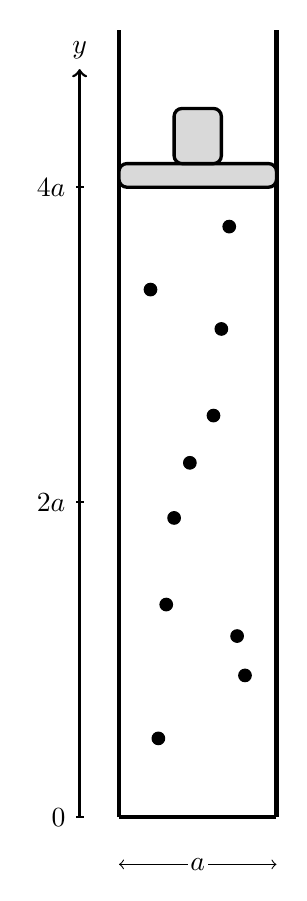
\begin{tikzpicture}[scale=1]

  % parameters
  \def\a{2}    % cylinder width
  \def\H{10}   % total height (>4a)
  \def\yplunger{8} % plunger position = 4a (a=2 => 4a=8)

  % cylinder walls
  \draw[line width=1.5pt] (0,0) -- (0,\H);
  \draw[line width=1.5pt] (\a,0) -- (\a,\H);
  \draw[line width=1.5pt] (0,0) -- (\a,0);

  % plunger at y=4a
  \draw[fill=gray!30, line width=1.2pt, rounded corners=0.1cm] 
      (0,\yplunger) rectangle (\a,\yplunger+0.3);

  % plunger handle (centered above plunger)
  \draw[fill=gray!30, line width=1.2pt, rounded corners=0.1cm] 
      (\a/2-0.3,\yplunger+0.3) rectangle (\a/2+0.3,\yplunger+1.0);

  % label the width a
  \draw[<->] (0,-0.6) -- (\a,-0.6)
      node[midway,fill=white,inner sep=1pt] {$a$};
  
  % gas molecules
  \foreach \x/\y in {0.5/1,1.5/2.3,0.7/3.8,1.2/5.1,0.4/6.7,
                     1.6/1.8,0.9/4.5,1.3/6.2,0.6/2.7,1.4/7.5} {
    \draw[fill=black] (\x,\y) circle (0.08);
  }

  % draw y-axis and ticks:
  \draw[->, line width=1pt] (-0.5,0) -- (-0.5,\H-0.5) node[above] {$y$};
  \draw[thick] (-0.45,0) -- (-0.55,0) node[left, black] {$0$};
  \draw[thick] (-0.45,4) -- (-0.55,4) node[left, black] {$2a$};
  \draw[thick] (-0.45,8) -- (-0.55,8) node[left, black] {$4a$};
  
\end{tikzpicture}
\caption{A 2-D gas cylinder of width $a$, containing an ideal gas of
  $N$ particles.  The plunger initially located at $y=4a$ is used to
  compress the gas.}
\label{fig:cgas}
\end{figure}


Consider the 2-D gas column showin in Fig.~\ref{fig:cgas}.  When the
column is at heigh $h$ the area of the gas is $A = a h$.  In the
isothermal case, the temperature remains at $T=T_1$.  So the ideal gas
law (as written in Equation~\ref{eqn:iglaw}) becomes:
\begin{equation}
\label{eqn:oiso}
\frac{O}{O_0} = \left( \frac{T_1}{T_0} \right) \left( \frac{a}{h} \right) 
\end{equation}
If the piston is initially at $y=h_1$ and we compress it until $y=h_2$, we have, in our system of units:
\begin{equation}
\label{eqn:wiso}
\frac{W}{U_0} = \frac{T}{T_0} \; \ln \; \left( \frac{h_1}{h_2}\right)
\end{equation}
and in our program we would calculate the work as
\begin{python}
def work_iso(T, hi, hf)
     return T * np.log(hi/hf)
\end{python}

\section{Adiabatic Compression}

During an adiabatic process, no thermal energy enters or leaves the gas, so
$$Q = 0$$
The total energy can still change by work done on the gas, with:
$$\Delta U = Q + W = W$$
Adiabatic processes are generally more difficult to calculate than
isothermal because many macroscopic state properties change
simultaneously: U,T,P and V.  The one simplification we have is that
$$dU = dW = - P dV$$
From:
$$U = \frac{f}{2} N k T$$
and so:
$$\frac{f}{2} N k dT = -P dV$$
dividing by the ideal gas we obtain:
$$\frac{f}{2} \frac{dT}{T} = - \frac{dV}{V}$$
Integrating both sides we obtain:
\begin{eqnarray*}
\int \frac{f}{2} \frac{dT}{T} &=& - \int \frac{dV}{V} \\
\frac{f}{2} \ln(T) &=& -\ln(V) + C \\
\ln\left( T^{f/2}\;V \right) &=& C \\
T^{f/2}\;V &=& C \\
T\;V^{2/f} &=& C \\
\end{eqnarray*}
Using the ideal gas law to write $T$ in terms of $P$ and $V$ we obtain:
$$P\;V^{((f+2)/f} = C $$

In the case of 2-D gas with initial pressure $O_1$ and area $A_1$ the
pressure $O$ and area $A$ during adiabatic compression or expansion is
given by:
$$ O A^2 = O_1 A_1^2 $$
The work done compressing the gas from $A_1$ to $A_2$ is:
\begin{eqnarray*}
W &=& - \int_{A_1}^{A_2} O(A) \; dA \\
  &=& - O_1 A_1^2 \int_{A_1}^{A_2} \frac{dA}{A^2} \\
  &=&  O_1 A_1^2 \; \left. \frac{1}{A} \; \right|_{A_1}^{A_2} \\
  &=&  O_1 A_1   \; \left( \frac{A_1}{A_2} - 1 \right) \\
  &=&  N k T_1  \; \left( \frac{A_1}{A_2} - 1 \right) \\
\end{eqnarray*}

For the case of the gas cylinder shown in Fig.~\ref{fig:cgas}, with
height of the column initially at $h_1$, the pressure during adiabatic
compression is given by:
\begin{equation}
\label{eqn:oadi}
\frac{O}{O_0} = \left( \frac{T_1}{T_0} \right) \left( \frac{a h_1}{h^2} \right) 
\end{equation}
and the work done compressing the gas until the height is $h_2$ is:
\begin{equation}
\label{eqn:wadi}
\frac{W}{U_0} = \frac{T_1}{T_0} \left( \frac{A_1}{A_2} - 1 \right)
\end{equation}

\section{Collision Model}

\begin{figure}[htbp]
  \begin{center}
\begin{tikzpicture}

  % Blue horizontal arrows
  \draw[->, line width=1.5pt, blue] (-3,0) -- (-0.1,0);
  \draw[->, line width=1.5pt, blue] (3,0)  -- (0.1,0);

  % Red slanted arrows
  \draw[->, line width=1.5pt, red]  (0,0) -- (3*0.50,3*0.86) coordinate (A);
  \draw[->, line width=1.5pt, red]  (0,0) -- (-3*0.50,-3*0.86) coordinate (B);

  % Angle label
  \node[right] at (0.5,0.5) {$\theta$};

  % Horizontal vector labels
  \node[left]  at (-3,0) {a};
  \node[right] at (3,0)  {b};

  % Slanted vector labels at arrow tips
  \node[above] at (A) {a};
  \node[below] at (B) {b};

  % Midpoint labels for horizontal arrows
  \node[above] at (-1.5,0) {$\vec{u}$};
  \node[above] at (1.5,0)  {$-\vec{u}$};

  % Midpoint labels for slanted arrows
  \node[left] at (0.8,1.5)  {$\vec{w}$};
  \node[left] at (-0.8,-1.4) {$-\vec{w}$};

\end{tikzpicture}
\caption{The collision model in the center-of-mass:  incoming molecule $a$ with velocity $\vec{u}$ collides with the incoming particle $b$ of identical mass with velocity $-\vec{u}$.  Particle $a$ is scattered by angle $\theta$ and leaves with velocity $\vec{w}$, while particle $b$ leaves with velocity $\vec{w}$.  The magnitude of the final and initial velocities are the same:  $|\vec{u}| = |\vec{w}|$.}
\label{fig:collcms}
\end{center}
\end{figure}

\noindent
At the heart of your numerical simulation is the collision model.  It
is the collisions of molecules that will allow your simulated gas to
reach thermal equilibrium.  We will use the simple elastic collision
of identical mass particles, as illustrated in Fig.~\ref{fig:collcms},
as our collision model.  We consider particles a and b with velocities
$\vec{v_a}$ and $\vec{v_b}$ in the lab frame.  The velocity of
particle a in the CMS frame before the collision is
\begin{displaymath}
\vec{u} = \frac{\vec{v_a} - \vec{v_b}}{2}.
\end{displaymath}
and the velocity of particle b is $-\vec{u}$.

The collision rotates the velocity of particle a by the scattering
angle $\theta$ so that the velocity $\vec{w}$ after the collision is
\begin{displaymath}
\begin{pmatrix}
w_x \\
w_y \\
\end{pmatrix}
  =
\begin{pmatrix}
\cos \theta  & -\sin \theta \\
\sin \theta  & \cos \theta \\
\end{pmatrix}
\,
\begin{pmatrix}
u_x \\
u_y \\
\end{pmatrix}
\end{displaymath}
The velocity of particle b after scattering is $-\vec{w}$.

In the lab frame, the velocity of molecule a changes by an amount:
\begin{displaymath}
\Delta \vec{v_a} = \vec{w} - \vec{u}  
\end{displaymath}
and the velocity of molecule b changes by an amount:
\begin{displaymath}
\Delta \vec{v_b} = (-\vec{w}) - (-\vec{u}) = -\Delta \vec{v_a}
\end{displaymath}

Our Python implementation for the collision will be computed in terms
of the components of the velocity vectors of molecule a and molecule
b:
\begin{eqnarray*}
\vec{v_a} &=& 
\begin{pmatrix}
a_x \\
a_y \\
\end{pmatrix} \\
\vec{v_b} &=& 
\begin{pmatrix}
b_x \\
b_y \\
\end{pmatrix} \\
\end{eqnarray*}
We'll use the Python variable names {\tt ax}, {\tt ay}, {\tt bx}, and
{\tt by} to refer to $a_x$, $a_y$, $b_x$, and $b_y$.

You will implement the collision model as a Python function:
\begin{python}
def collide(ax,ay,bx,by,theta):
    # your code here
    return ax, ay, bx, by # updated values
\end{python}
which takes the lab frame veclocitys of particle a (ax,ay) and b (bx,
by) and returns the lab frame velocities after scattering by an angle
theta.  {\bf Please stick to these variable names and function
  definition in your own program}.  It will help us help you debug
your code.

To implement the algorithm, first calculate the $x$ and $y$ component
of $\vec{u}$ as:
\begin{eqnarray*}
u_x &\equiv& \frac{a_x - b_x}{2} \\
u_y &\equiv& \frac{a_y - b_y}{2} \\
\end{eqnarray*}
Then compute the $x$ and $y$ component to the change in velocity of particle a and particle b:
\begin{eqnarray*}
  \Delta a_x &=& (\cos\theta - 1) \, u_x - \sin\theta \, u_y \\
  \Delta a_y &=& (\cos\theta - 1) \, u_y + \sin\theta \,  u_x \\
\end{eqnarray*}
Finally, update the $x$ and $y$ components of the particle velocities to their value after the collision:
\begin{eqnarray*}
  a_x &\to& a_x + \Delta a_x \\
  a_y &\to& a_y + \Delta a_y \\
  b_x &\to& b_x - \Delta a_x \\
  b_y &\to& b_y - \Delta a_y \\
\end{eqnarray*}
Some test values with known answers are provided in the homework
section.  Make sure your collision model is rock solid before trying
anything else!

\section{Thermal Equilibrium of a Molecular Dynamics Model}


\begin{figure}[htbp]
\begin{center}
  {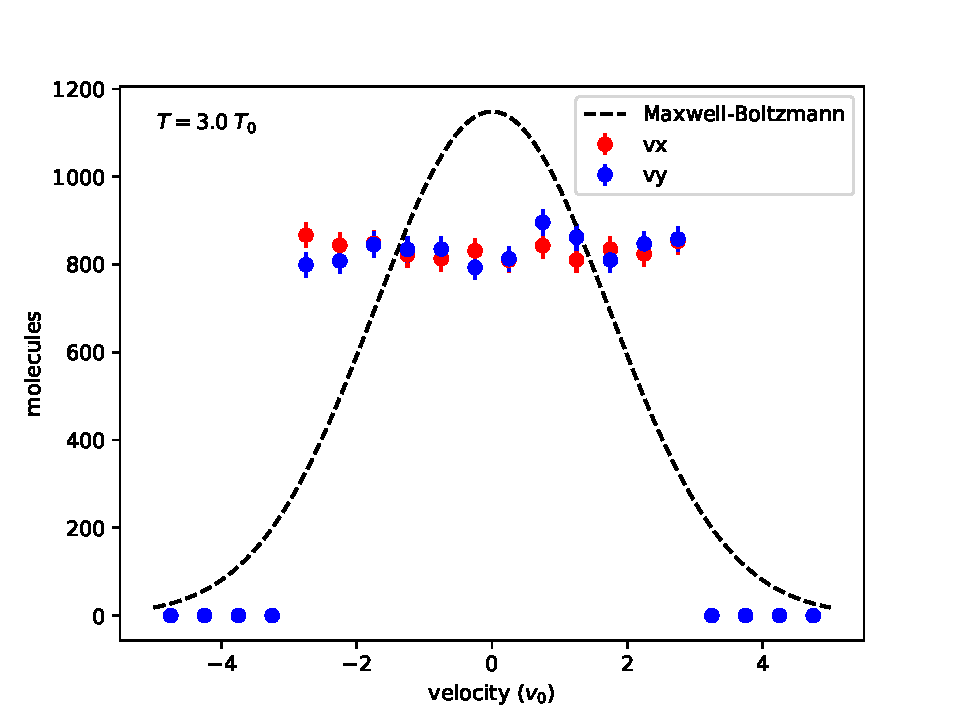
\includegraphics[width=0.70\textwidth]{plots/vinit.pdf}}
\end{center}
\caption{\label{fig:vinit} Velocity distribution immediately after initialization.}
\end{figure}

Our model will consist of $N=10000$ molecules constrained to a 2-D
cylinder of width $a$ and initial height $H = 4 a$.  We will track
both components of each particles velocity $v_x$ and $v_y$, but we
will only track the particles $y$ position.  Nothing we are doing will
depend on the $x$ position, so we do not track it: we can imagine each
particle bouncing off the side walls as needed to stay in position.
In python, this would be coded as:
\begin{python}
NGAS=10000
H  = 4
VM
vx = np.random.uniform(size=NGAS, low=-3, high=3)
vy = np.random.uniform(size=NGAS, low=-3, high=3)
y  = np.random.uniform(size=NGAS, low= 0, high=H)
\end{python}
After calling this code, the distribution in each variable can be
displayed as a histogram, as in the following snippet:
\begin{python}
hvx,bins = np.histogram(vx,bins=20,range=(-5,5))
cbins = (bins[1:]+bins[:-1])/2
plt.errorbar(cbins, hvx,fmt="ro", yerr=np.sqrt(hvx),label="vx")
\end{python}

\begin{figure}[htbp]
\begin{center}
  {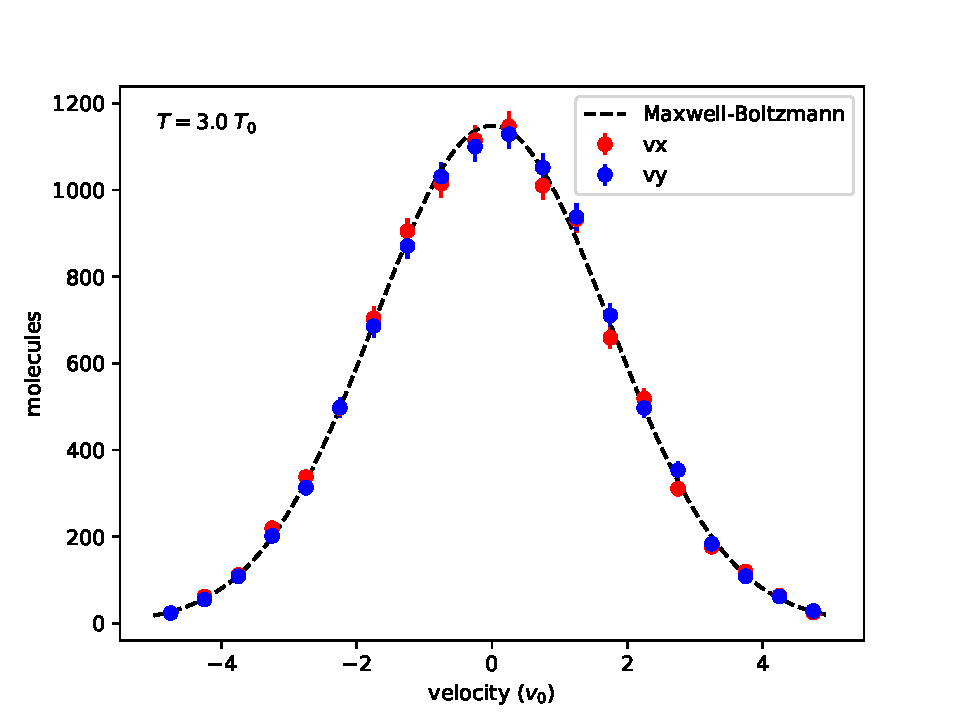
\includegraphics[width=0.70\textwidth]{plots/vself.pdf}}
\end{center}
\caption{\label{fig:vself} Thermal equilibrium.}
\end{figure}

Immediately after initialization, as shown in Fig.~\ref{fig:vinit} the
gas is not in thermal equilibrium, due to our non-physical
initialization of the momenta.  We will use our simple collision model
to allow the gas to reach equilibrium.  Too keep things simple, we won't insist on physical proximity (the $y$ values) in order to collide particles.  We'll simply choose pairs at random, such as with:
\begin{python}
a,b = np.random.choice(NGAS,size=2, replace=False)
\end{python}
and collide particles $a$ and $b$ by updating their $v_x$ and $v_y$
coordinates using the collision function and a randomly choosen value
of $\theta$.  After 100k collisions, the system reaches thermal
equilibrium, as shown in Fig.~\ref{fig:vself}.

The temperature of the gas remains the same, however, as the
collisions conserve energy.  In order to set the temperature, we will
let the system reach thermal equilibrium with a reservoir at the
desired temperature.  To simulated this process, we'll draw random
values from the Maxwell-Boltzmann distribution of the velocity
components:
\begin{python}
Tr = 1
rx = np.random.normal(0,np.sqrt(Tr),size=n)
ry = np.random.normal(0,np.sqrt(Tr),size=n)
\end{python}
and collide these $n$ reservoir particles with another $n$ randomly
choosen gas particles.  Each reservoir particle should be used for one
collision only and then discarded, to simulate an infinitely large
reservoir.


\section{Bouncing and Compression}

Our numerical model includes the $y$-position of each molecules.  While inside the container, the molecules position can be updated for a time step $\Delta t$ as:
$$y \to y + v_y \Delta t$$
This is fine, for as long as the particles remain within the container.  However, particles with negative $v_y$ will eventually be updated to have $y < 0$.  These particles are bounced back into the container by the simple update:
\begin{equation}
y \to -y  
\end{equation}
and
\begin{equation}
v_y \to -v_y.  
\end{equation}
Meanwhile, particles moving upward will eventually be updated to have
$y > h$, where $h$ is the current location of the plunger.  In this case, the particles are bounced back in by the update:
\begin{equation}
y \to 2h - y  
\end{equation}
If the piston is stationary, the velocities are updated as:
\begin{equation}
v_y \to -v_y.  
\end{equation}
However, we'll need to model a moving piston during compression.

\begin{figure}[htbp]
  \begin{center}
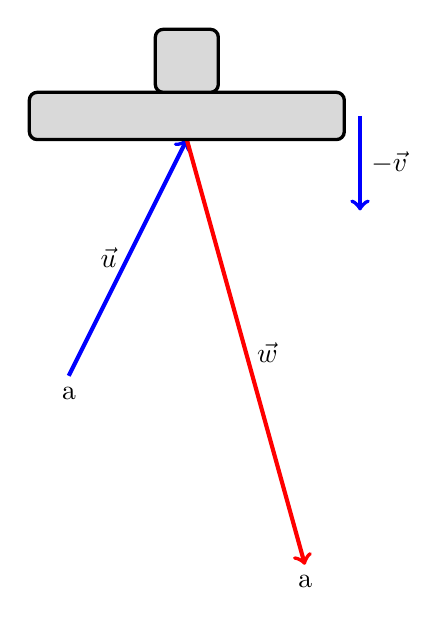
\begin{tikzpicture}[scale=1]

  % Parameters
  \def\a{4}             % width of plunger
  \def\yplunger{3}      % y-position of plunger
  \def\plungerheight{0.6}

  \draw[->, line width=1.5pt, blue] (0.5,0) -- (2,\yplunger)
  node[black, midway, left] {$\vec{u}$}
  node[pos=0, below, text=black] {a};

  \draw[->, line width=1.5pt, red] (2,\yplunger) -- (3.5,-2.4)
  node[black, midway, right] {$\vec{w}$}
  node[pos=1, below, text=black] {a};

  
  % Draw the plunger (rectangle + handle)
  \draw[fill=gray!30, line width=1.2pt, rounded corners=0.1cm] 
      (0,\yplunger) rectangle (\a,\yplunger+\plungerheight);
  \draw[fill=gray!30, line width=1.2pt, rounded corners=0.1cm] 
      (\a/2-0.4,\yplunger+\plungerheight) rectangle (\a/2+0.4,\yplunger+\plungerheight+0.8);

  % Plunger velocity label
  \draw[->, line width=1.5pt, blue] (\a+0.2,\yplunger+\plungerheight/2) -- ++(0,-1.2)
  node[black, midway, right] {$-\vec{v}$};

  % Label plunger velocity
  %\node[right] at (\a+0.2,\yplunger+\plungerheight/2) {$v_p$};
\end{tikzpicture}    
    \caption{Gas particle a at velocity $\vec{u}$ collides with the plunger, travelling downward with velocity $-\vec{v}$, and recoils with new velocity $\vec{w}$.}
\label{fig:bounce}
\end{center}
\end{figure}

\noindent
During compression, molecules strike the moving plunger and recoil, as
illustrated in Fig.~\ref{fig:bounce}.  The particle $a$ has initial
velocity $\vec{u}$.  After striking the plunger it recoils with new
velocity $\vec{w}$.  Your model will need to accurately simulate these
collisions.  The $x$-component of velocity is unchanged during the
collision:
$$w_x = u_x$$
and we don't model the $x$-position of molecules.  The $y$-component of the velocity after the collision with the plunger is given by:
\begin{equation}
\label{eqn:mpiston}
w_y = -u_y + 2 \, v_y
\end{equation}
Note carefully that a piston moving down, as for compression, will have $v_y < 0$.


\section{Homework Problems}

\noindent
{\bf Please submit one PDF file (including output) and one python
  notebook file (.ipynb) of your completed assignment.}  If using
C/C++, submit text or PDF of your output and the source code.


{\bf Zero credit if you do not use our system of units consistently!}
When I ask you to calculate a quantity, e.g. temperature, I want the
answer in our units, e.g. $T_0$.  Do not first calculate in SI units
and then convert!

\noindent
{\bf Problem 1:} Implement the collision model described in the text.
Test your code with some simple cases first, rotations by
zero,quarter,half,and three quarters of a full turn:
\begin{python}
tau = 2*np.pi # Using 2 pi is like saying twice half-way...
# lab frame is cms, incoming on x axis:
print(np.around(collide(1,0,-1,0,0),2)+0)
print(np.around(collide(1,0,-1,0,tau/4),2)+0)
print(np.around(collide(1,0,-1,0,tau/2),2)+0)
print(np.around(collide(1,0,-1,0,3*tau/4),2)+0)
\end{python}
which should have the output:
\begin{verbatim}
[ 1.  0. -1.  0.]
[ 0.  1.  0. -1.]
[-1.  0.  1.  0.]
[ 0. -1.  0.  1.]
\end{verbatim}
And:
\begin{python}
# lab frame is cms, incoming on	y axis:
print(np.around(collide(0,1,0,-1,0),2)+0)
print(np.around(collide(0,1,0,-1,tau/4),2)+0)
print(np.around(collide(0,1,0,-1,tau/2),2)+0)
print(np.around(collide(0,1,0,-1,3*tau/4),2)+0)
\end{python}
which should have the output:
\begin{verbatim}
[ 0.  1.  0. -1.]
[-1.  0.  1.  0.]
[ 0. -1.  0.  1.]
[ 1.  0. -1.  0.]
\end{verbatim}
Then test your collision function where the lab frame is not the CMS frame:
\begin{python}
# boost along x axis, incoming on y axis:
print(np.around(collide(1,1,1,-1,0),2)+0)
print(np.around(collide(1,1,1,-1,tau/4),2)+0)
print(np.around(collide(1,1,1,-1,tau/2),2)+0)
print(np.around(collide(1,1,1,-1,3*tau/4),2)+0)
\end{python}
which should output:
\begin{verbatim}
[ 1.  1.  1. -1.]
[0. 0. 2. 0.]
[ 1. -1.  1.  1.]
[2. 0. 0. 0.]
\end{verbatim} \vskip 0.25cm
Finally, test your collision function with randomly choosen values:
\begin{python}
# test with random values:
print(np.around(collide(6.24, 1.78, 3.35, 5.98, 3.19),2))
print(np.around(collide(4.07, 4.69, 1.61, 4.54, 2.46),2))
print(np.around(collide(5.28, 2.99, 4.77, 5.22, 3.15),2))
print(np.around(collide(2.84, 5.37, 5.47, 6.16, 1.59),2))
\end{python}
which should output:
\begin{verbatim}
[3.25 5.91 6.34 1.85]
[1.84 5.33 3.84 3.9 ]
[4.76 5.22 5.29 2.99]
[4.58 4.46 3.73 7.07]
\end{verbatim}
Being able to Develop good testing regimens is an essential program skill.\\[3pt] 


\noindent
{\bf Problem 2:} Initialize the numerical model as described in the text, and reproduce Fig.~\ref{fig:vinit}.  Calculate the temperature.\\[3pt]

\noindent
{\bf Problem 3:} By applying your collision model to randomly choosen molecules 100,000 times, bring your model to thermal equilibrium and reproduce Fig.~\ref{fig:vself}. Calculate the temperature.\\[3pt]

\noindent
{\bf Problem 4:}  Bring your model into thermal equilibrium with a reservoir at $T = 1 T_0$.
Apply your collision model to a radomly choosen gas molecule and a randomly drawn reservoir particle, as described in the text, 100,000 times.  Plot the resulting histogram, as in the previous problems.  Calculate the temperature.  It should match the reservoir!\\[3pt]

\noindent
{\bf Problem 5:}
Simulate pressure with the gas at $T = 1 T_0$ and the plunger {\bf
  stationary} at $h=4a$.  Update the $y$ position of each molecule for
a time interval $\Delta t = 10 \tau$.  Handle bouncing at both $y=h$ and $y=0$.
Keep track of the total $\Delta v_y$ for particles bounced at the piston.
In our system of units, the presure can be calculated as:
$$\frac{O}{O_0} = \frac{1}{N}\frac{\Delta v_y}{v_0} \frac{\tau}{\Delta t}$$.
Compare yours simulated pressure with your expectation from Equation~\ref{eqn:iglaw}.\\[3pt]

\noindent
{\bf Problem 6:}
Simulate isothermal compression of the gas from $h=4a$ to $h=2a$ in 20
timesteps of size $\Delta t = 10 \tau$.  Set the speed of the piston
appropriately.  Repeat the pressure calculation from the previous
problem at each step, updating the location of the piston before each
step, and accounting for its speed in the momentum transferred to
bouncing molecules, as in Equation~\ref{eqn:mpiston}.  Simulate an
isothermal process by bringing the system into thermal equilibrium
with a reservoir at $T = 1 T_0$ after each step.  Plot your measured
$O$ versus $A$ and compare to your expectation from
Equation~\ref{eqn:oiso} Integrate your curve to get the work done, and
compare to your expectation from Equation~\ref{eqn:wiso}\\[3pt]

\noindent
{\bf Problem 7:}
Simulate adiabatic compression of the gas from $h=4a$ to $h=2a$ in 80
timesteps of size $\Delta t = 10 \tau$.  Set the speed of the piston
appropriately.  Repeat the pressure calculation as in the previous
problem.  The collisions with the piston bring the gas out of thermal
equilibrium at each step.  This is an adiabatic process, so you cannot
use a reservoir.  Instead, bring the system into thermal equilibrium
by colliding pairs of particles as in Problem 2.  Plot your measured
$O$ versus $A$ and compare to your expectation from
Equation~\ref{eqn:oadi} Integrate your curve to get the work done, and
compare to your expectation from Equation~\ref{eqn:wadi}.\\[3pt]




\end{document}
